\documentclass[a4paper,12pt]{article}
\usepackage[english,ukrainian,russian]{babel}
\linespread{1}
\usepackage{ucs}
\usepackage[utf8]{inputenc}
\usepackage[T2A]{fontenc}
\usepackage[paper=portrait,pagesize]{typearea}
\usepackage{amsmath}
\usepackage{bigints}
\usepackage{amsfonts}
\usepackage{graphicx}
\usepackage{amssymb}
\usepackage{cancel}
\usepackage{gensymb}
\usepackage{multirow}
\usepackage{rotate} 
\usepackage{pdflscape}
\usepackage{bigstrut}
\usepackage[pageanchor]{hyperref}
\usepackage{chngpage}
\usepackage{fancybox,fancyhdr}
\newcommand\tab[1][1cm]{\hspace*{#1}}
\newcommand{\RomanNumeralCaps}[1]{\MakeUppercase{\romannumeral #1}}
\usepackage[left=20mm, top=20mm, right=15mm, bottom=15mm, nofoot]{geometry}


\begin{document}
    \pagestyle{fancy}
    \fancyhead{}
    \fancyhead[R]{ФІ-12 Завалій Олександр}
    \begin{center}
        \large{\textbf{Міністерство освіти і науки України\\
                Національний технічний університет України\\
                «Київський політехнічний інститут імені Ігоря Сікорського»\\
                Навчально-науковий Фізико-технічний інститут}}\\
        \hfill \break \hfill \break \hfill\break \hfill \break \hfill \break \hfill \break \hfill \break
        \hfill \break \hfill \break \hfill \break
        \begin{center}
            \normalsize{\textbf{ОПЕРАЦІЙНІ СИСТЕМИ\\
            Комп’ютерний практикум\\
            Робота №4}}
        \end{center}
    \end{center}
    \hfill \break \hfill \break \hfill \break \hfill \break \hfill \break \hfill \break \hfill \break
    \hfill \break \hfill \break \hfill \break \hfill \break 
    \begin{flushright}
        \large{ \hspace{35pt} Виконав:\\
            студент групи ФI-12\\
            Завалій Олександр\\} 
        \large{ \hspace{35pt} Перевірив:\\
        Кірієнко О.В.} 
    \end{flushright}
    \hfill \break \hfill \break \hfill \break \hfill \break \hfill \break \hfill \break \hfill \break
    \hfill \break
    \begin{center} \textbf{Київ-2023} \end{center}
    \thispagestyle{empty}

\newpage
    \begin{center}
        \section*{\bfseries{Робота №4.\\
        Розробка сценаріїв командної оболонки}}
    \end{center}
    \textbf{Мета:} \\
    \hangindent=1.5cm 
    \hangafter=+1 \noindent
    Оволодіння практичними навичками професійної
    роботи з командною оболонкою shell – використання
    змінних і створення командних файлів. \\
    \begin{center}
        \Large{Варіант №5}
    \end{center}
    Зміст індивідуального завдання:
    \begin{enumerate}
        \item Написати сценарій для оболонки bash згідно таких вимог:
        \begin{itemize}
            \item Сценарій перевіряє активність заданого користувача. Якщо користувач працює на комп’ютері, сценарій видає йому привітання. Якщо користувач не працює (немає
            логіну), сценарій повинен автоматично згенерувати і відправити повідомлення електронної пошти на адресу начальника (можете обрати адресу на свій смак).
            \item Повідомлення повинно містити формальне вибачення і причину відсутності на роботі. Причина має обиратися рандомно з файлу, що містить щонайменше десять таких
            причин (наприклад, викликали до школи через погану поведінку сина, чекаєте на сантехніка бо трубу прорвало, тощо). Жодних натяків на втому чи головний біль! 
            Примітка: почуття гумору вітається, але завданням роботи все ж є написання сценарію, що працює, а не вправи у красному письменстві!
        \end{itemize}
        \item Налаштувати періодичний запуск сценарію за допомогою cron по понеділках о 9-й годині ранку.
    \end{enumerate}

\newpage
    \begin{center}
        \Large{Task \RomanNumeralCaps{1}}
    \end{center}
    \textbf{Написати сценарій для оболонки bash згідно таких вимог:}
    \begin{itemize}
        \item Сценарій перевіряє активність заданого користувача. Якщо користувач працює на комп’ютері, сценарій видає йому привітання. Якщо користувач не працює (немає
        логіну), сценарій повинен автоматично згенерувати і відправити повідомлення електронної пошти на адресу начальника (можете обрати адресу на свій смак).
        \item Повідомлення повинно містити формальне вибачення і причину відсутності на роботі. Причина має обиратися рандомно з файлу, що містить щонайменше десять таких
        причин (наприклад, викликали до школи через погану поведінку сина, чекаєте на сантехніка бо трубу прорвало, тощо). Жодних натяків на втому чи головний біль! 
        Примітка: почуття гумору вітається, але завданням роботи все ж є написання сценарію, що працює, а не вправи у красному письменстві!
    \end{itemize}
    \begin{minipage}[h]{1\linewidth}
        \centering
        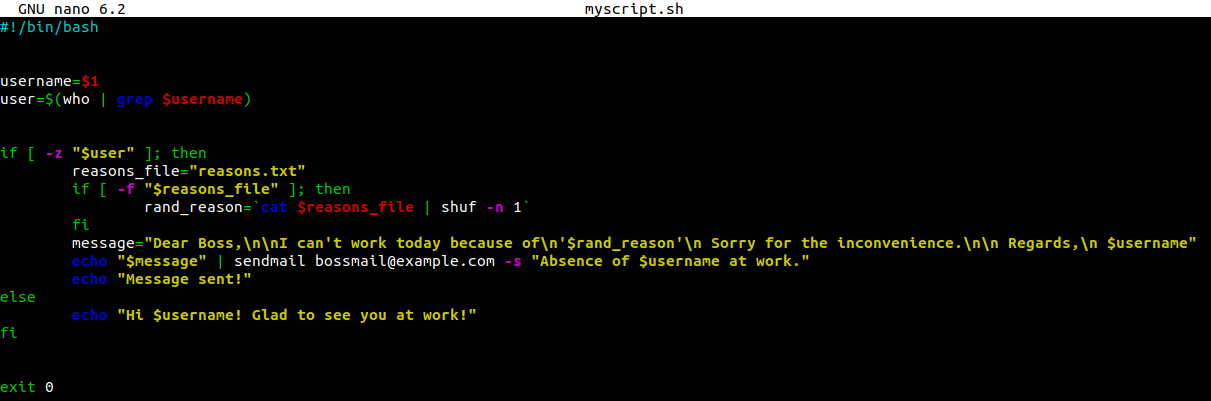
\includegraphics[width=0.9\linewidth]{Prt sc/Figure_1.png}  
    \end{minipage}
    \begin{minipage}[h]{1\linewidth}
        \centering
        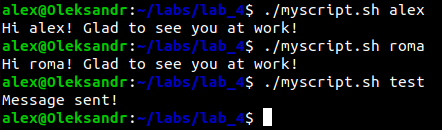
\includegraphics[width=0.9\linewidth]{Prt sc/Figure_2.png}  
    \end{minipage}
    \begin{minipage}[h]{1\linewidth}
        \centering
        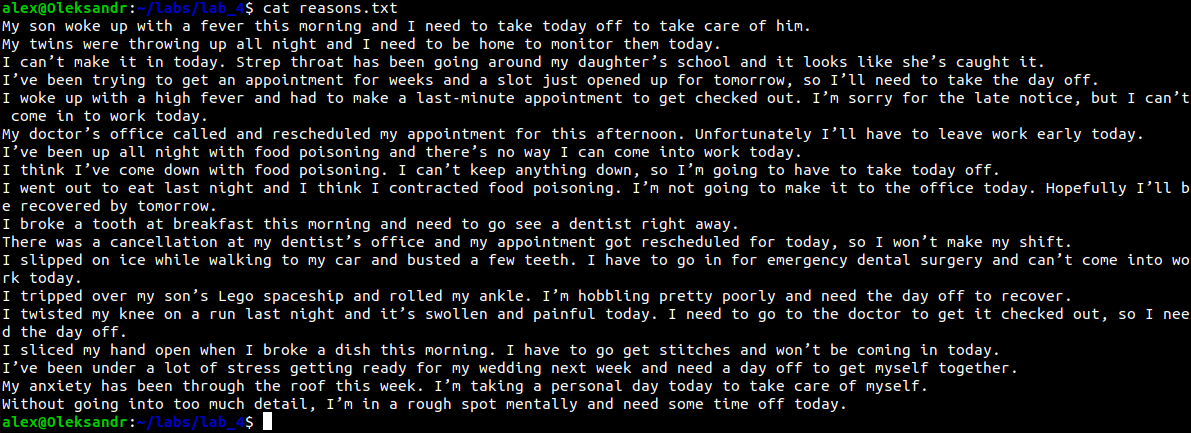
\includegraphics[width=0.9\linewidth]{Prt sc/Figure_3.png}  
    \end{minipage}

\newpage
    \begin{center}
        \Large{Task \RomanNumeralCaps{2}}
    \end{center}
    \textbf{Налаштувати періодичний запуск сценарію за допомогою cron по понеділках о 9-й годині ранку.} \\
    \begin{minipage}[h]{1\linewidth}
        \centering
        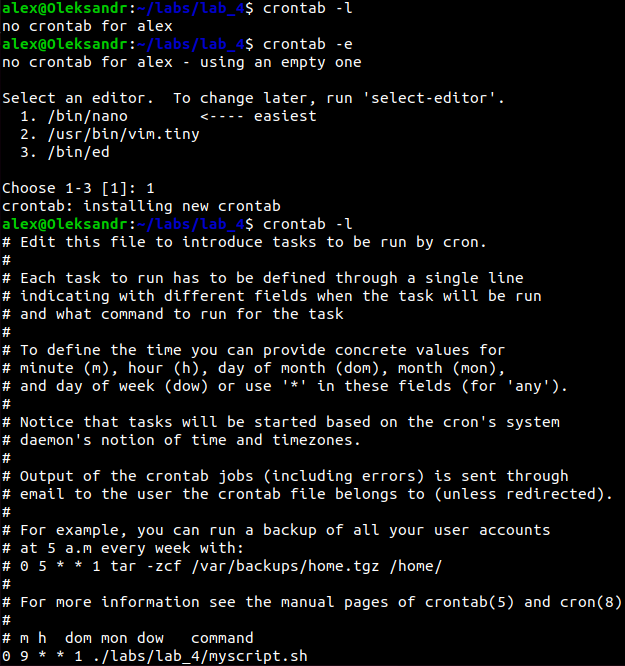
\includegraphics[width=0.9\linewidth]{Prt sc/Figure_4.png}  
    \end{minipage}
\end{document}